

\chapter{Introducción}

\section{Alcance}

El objetivo de este trabajo es desarrollar un escenario didáctico que permita a los analistas de ciberseguridad mejorar sus capacidades de detección e investigación mediante la comprensión del proceso completo de creación de un ciberataque. El resultado final del proyecto será un conjunto de artefactos forenses de los sistemas infectados, que servirá como base para ejercicios de análisis forense (blue team).

Para generar dicho recurso, el núcleo del trabajo se centrará en la concepción, diseño y desarrollo de un ciberataque realista, su ejecución controlada en un sistema víctima y la documentación íntegra del proceso ofensivo llevado a cabo. De este modo, quien reciba los artefactos forenses podrá analizar la infección desde el punto de vista del analista forense, pero también interpretar las acciones del atacante, entendiendo mejor el cómo y el porqué de cada artefacto encontrado.

En definitiva, este trabajo busca aproximar al analista a la mentalidad del atacante, con el fin de reforzar sus habilidades de detección, interpretación y respuesta ante amenazas reales.

\section{Justificación}

Este trabajo se sitúa dentro del ámbito de la \textit{simulación de adversarios} (\textit{Adversary Simulation}), una metodología que permite evaluar de forma controlada tanto la eficacia de los sistemas de defensa como las capacidades del personal ante incidentes de seguridad. 

Aunque esta técnica puede aplicarse para probar sistemas, en este caso concreto el enfoque principal es la formación del personal. Se utiliza un escenario de ataque realista para que los analistas practiquen la detección, el análisis y la interpretación de un incidente completo, mejorando sus habilidades y comprensión del comportamiento de un atacante.

\section{Contribución}

Este trabajo presenta un escenario de ataque completo, documentado y reproducible para la formación práctica en análisis forense y respuesta a incidentes. Su principal aportación es la trazabilidad entre las acciones del atacante y las evidencias generadas, permitiendo relacionar cada artefacto forense con su origen técnico y comprender las decisiones adoptadas durante la intrusión.

A diferencia de los recursos formativos tradicionales, el escenario abarca todo el ciclo del ataque, desde el acceso inicial hasta la persistencia y el control remoto del sistema comprometido. Este enfoque integra la perspectiva ofensiva y defensiva, facilitando no solo la identificación de evidencias, sino también la comprensión de la intención detrás de cada técnica empleada.

En conjunto, el trabajo contribuye a reducir la brecha entre la teoría y la práctica, proporcionando a la comunidad académica un entorno realista para el estudio y análisis de incidentes de ciberseguridad.

\begin{figure}[h!]
    \centering
    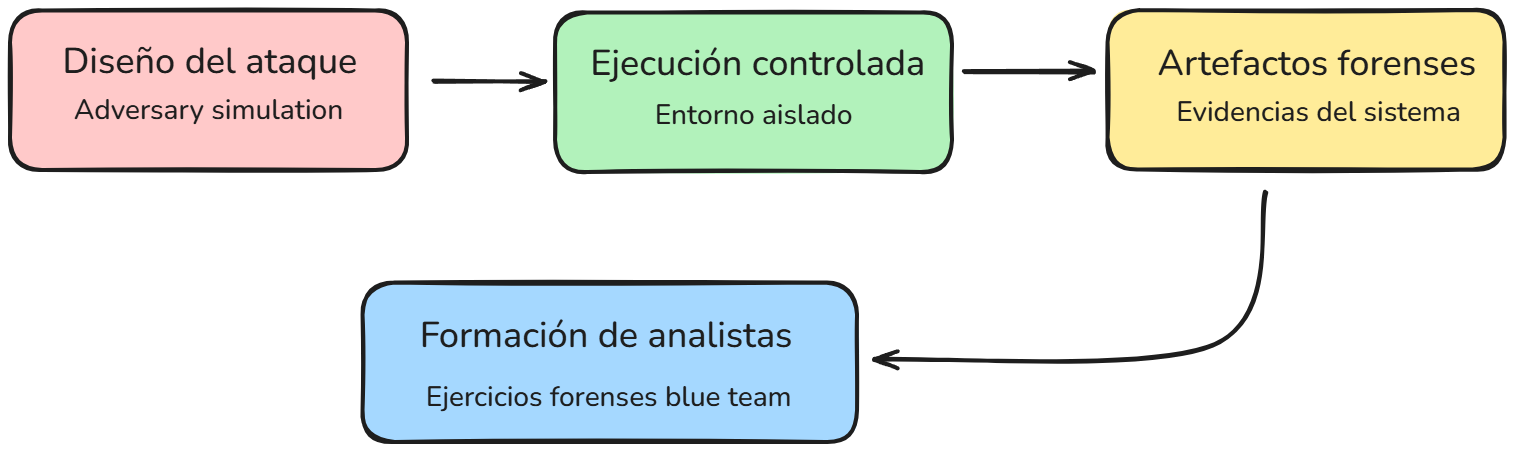
\includegraphics[width=0.8\textwidth]{figures/contribucion.png}
    \caption{Visión general del trabajo: a partir del diseño y ejecución controlada de un ciberataque, se generan los artefactos forenses que sirven como material de formación para analistas de seguridad.}
    \label{fig:contribucion}
\end{figure}
